\input{../../Plantillas-Fomato/Tareas/tarea.tex}
\cabe{Geometría 3: Tarea 5}{Jhonny Lanzuisi, 1510759}
\usetikzlibrary{arrows}
\pgfplotsset{compat=1.16}
\begin{document}
		\tituloD{Geometría  3}{Quinta Tarea}
		\subsection*{Ejercicio 1}
		\marginnote{
			\begin{minipage}{8cm}
				\begin{figure}[H]\hspace*{-2em}
					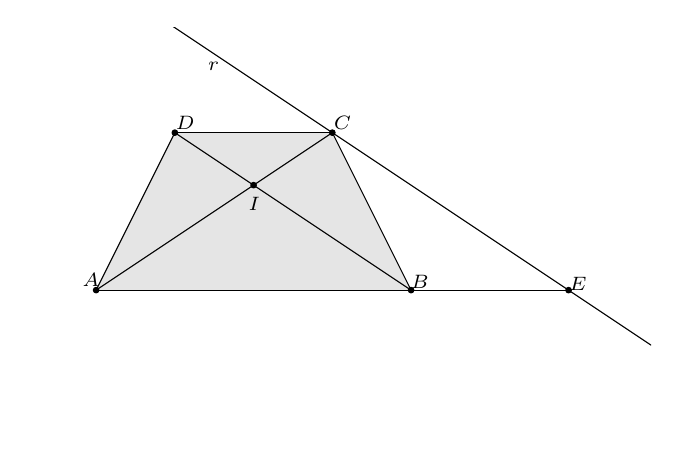
\begin{tikzpicture}[line cap=round,line join=round,>=triangle 45,x=1cm,y=1cm,scale=1]
					\clip(-0.8690146553979121,-2.0018549308798055) rectangle (7.047515007813354,3.3331976682408246);
					\fill[line width=0.4pt,fill=black,fill opacity=0.10000000149011612] (0,0) -- (4,0) -- (3,2) -- (1,2) -- cycle;
					\draw [line width=0.4pt] (0,0)-- (4,0);
					\draw [line width=0.4pt] (4,0)-- (3,2);
					\draw [line width=0.4pt] (3,2)-- (1,2);
					\draw [line width=0.4pt] (1,2)-- (0,0);
					\draw [line width=0.4pt] (1,2)-- (4,0);
					\draw [line width=0.4pt] (3,2)-- (0,0);
					\draw [line width=0.4pt,domain=-0.8690146553979121:7.047515007813354] plot(\x,{(--12-2*\x)/3});
					\draw [line width=0.4pt] (4,0)-- (6,0);
					\begin{scriptsize}
					\draw [fill=black] (0,0) circle (1pt);
					\draw[color=black] (-0.06588845768082716,0.124790460013902) node {$A$};
					\draw [fill=black] (4,0) circle (1pt);
					\draw[color=black] (4.113645836561146,0.10840012944824721) node {$B$};
					\draw [fill=black] (3,2) circle (1pt);
					\draw[color=black] (3.1302260026218582,2.124410789023785) node {$C$};
					\draw [fill=black] (1,2) circle (1pt);
					\draw[color=black] (1.130605673611973,2.124410789023785) node {$D$};
					\draw [fill=black] (2,1.3333333333333333) circle (1pt);
					\draw[color=black] (2.0074883588745043,1.1000151286703612) node {$I$};
					\draw[color=black] (1.4911929460563782,2.8373901686297676) node {$r$};
					\draw [fill=black] (6,0) circle (1pt);
					\draw[color=black] (6.121461330853858,0.08381463359976506) node {$E$};
					\end{scriptsize}
					\end{tikzpicture}
				\end{figure}
			\end{minipage}
		}
	Demostrar que las diagonales de un trapecio se dividen mutuamente en
	partes proporcionales a las bases
	\begin{sol}
		Sea $ABCD$ un trapecio y llamemos $I$ a la intersección de sus diagonales. Tomemos la paralela a la diagonal $DB$ que pasa por $C$ y llamemos $E$ a la intersección de dicha paralela con la prolongación de la base $AB$. Entonces la paralela $CE$ determina sobre las prolongaciones de los lados del triángulo $AIB$ segmentos proporcionales, esto es,
		\[ \frac{AB}{BE} = \frac{AI}{IC} \]
		pero como $BE = DC$ se tiene
		\[ \frac{AB}{DC} = \frac{AI}{IC}. \]
		Puede hacerse una construcción análoga tomando la paralela a la diagonal $AC$ por el punto $D$ para obtener
		\[ \frac{AB}{DC} = \frac{BI}{ID} = \frac{AI}{IC} \]
		que es lo que queríamos demostrar.
	\end{sol}

\subsection*{Ejercicio 2}
El segmento interior de la paralela a las bases de un trapecio por el
punto de intersección de las diagonales es bisectado por dicho punto.
Demostrar esta afirmación y calcular la longitud de un tal segmento en
función de las bases.
	\marginnote{
	\begin{minipage}{8cm}
		\begin{figure}[H]\hspace*{-1em}
			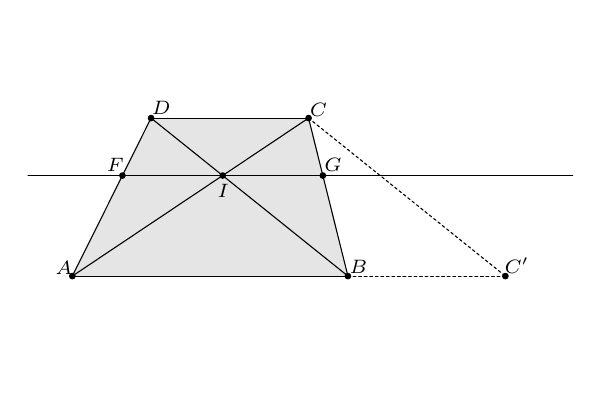
\begin{tikzpicture}[line cap=round,line join=round,>=triangle 45,x=1cm,y=1cm]

			\clip(-0.5670075110137496,-1.2412141628968727) rectangle (6.361522601105957,3.1549584521030583);

			\fill[line width=0.4pt,fill=black,fill opacity=0.10000000149011612] (0,0) -- (3.5,0) -- (3,2.0067529533256527) -- (1,2.0067529533256527) -- cycle;

			\draw [line width=0.4pt] (0,0)-- (3.5,0);

			\draw [line width=0.4pt] (3.5,0)-- (3,2.0067529533256527);

			\draw [line width=0.4pt] (3,2.0067529533256527)-- (1,2.0067529533256527);

			\draw [line width=0.4pt] (1,2.0067529533256527)-- (0,0);

			\draw [line width=0.4pt] (1,2.0067529533256527)-- (3.5,0);

			\draw [line width=0.4pt] (3,2.0067529533256527)-- (0,0);

			\draw [line width=0.4pt,domain=-0.5670075110137496:6.361522601105957] plot(\x,{(-28.18940190976861-0*\x)/-22.074282486582177});

			\draw [line width=0.4pt,dash pattern=on 1pt off 1pt] (3,2.0067529533256527)-- (5.5,0);

			\draw [line width=0.4pt,dash pattern=on 1pt off 1pt] (5.5,0)-- (3.5,0);

			\begin{scriptsize}

			\draw [fill=black] (0,0) circle (1pt);

			\draw[color=black] (-0.10780668486936351,0.09924707224519541) node {$A$};

			\draw [fill=black] (3.5,0) circle (1pt);

			\draw[color=black] (3.633329457542252,0.11275297889650088) node {$B$};

			\draw [fill=black] (3,2.0067529533256527) circle (1pt);

			\draw[color=black] (3.1268579581182965,2.1116271632897106) node {$C$};

			\draw [fill=black] (1,2.0067529533256527) circle (1pt);

			\draw[color=black] (1.127983773725087,2.1318860232666688) node {$D$};

			\draw [fill=black] (1.9090909090909094,1.2770246066617794) circle (1pt);

			\draw[color=black] (1.9180793128264568,1.0851782577904947) node {$I$};

			\draw [fill=black] (0.6363636363636366,1.2770246066617794) circle (1pt);

			\draw[color=black] (0.5472297877189518,1.4160729707474788) node {$F$};

			\draw [fill=black] (3.1818181818181825,1.2770246066617794) circle (1pt);

			\draw[color=black] (3.3091876979109203,1.409320017421826) node {$G$};

			\draw [fill=black] (5.5,0) circle (1pt);

			\draw[color=black] (5.645709548586767,0.13301183887345908) node {$C'$};

			\end{scriptsize}

			\end{tikzpicture}
		\end{figure}
	\end{minipage}
}
\begin{sol}
	Sean $ABCD$ un trapecio, $I$ la intersección de sus diagonales y $F,G$ los puntos de corte de la paralela a las bases por $I$ con el trapecio. Entonces
	\[ \frac{FI}{DC} = \frac{IA}{CA} = \frac{AB}{AB+DC} \]
	y similarmente,
	\[ \frac{IG}{DC} = \frac{BI}{DB} = \frac{AB}{AB+DC}, \]
	por lo que $FI=IG$ y el punto $I$ bisecta al segmento $FG$.
	
	Sea $a=DC$ y $b=AB$ entonces
	\[ FG = 2a\frac{b}{b+a} = \frac{2ab}{a+b} = \frac{2}{\dfrac{1}{a} + \dfrac{1}{b}} \]
	que es la media ármonica de $a$ y $b$.
\end{sol}
\subsection*{Ejercicio 3}
	Dado un triángulo acutángulo, mostrar que el ortocentro $H$ y el baricentro $G$ estan separados armónicamente por el centro $N$ de la circunferencia de Feuerbach y el circuncentro $O$ de triángulo.
	\marginnote{
		\begin{minipage}{8cm}
			\begin{figure}[H]\hspace*{-5em}
				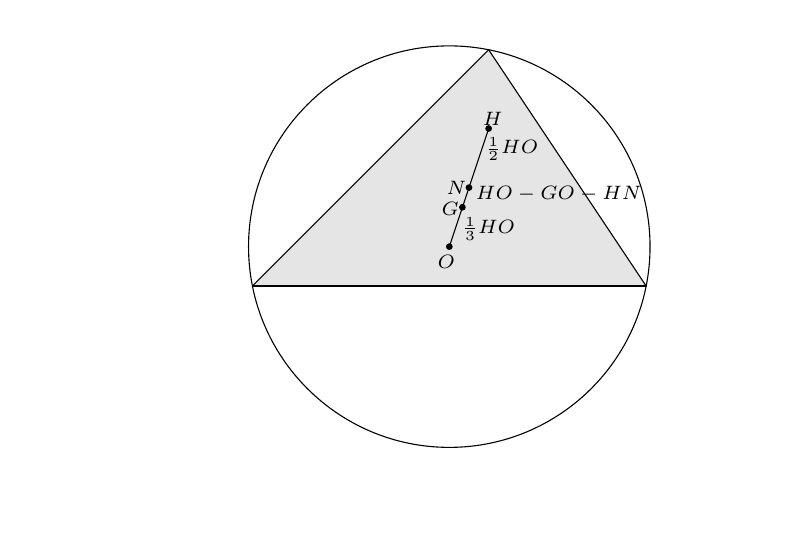
\begin{tikzpicture}[line cap=round,line join=round,>=triangle 45,x=1cm,y=1cm]

				\clip(-2.8545232036329473,-3.1062446535269266) rectangle (6.701391317102413,3.280716694521031);

				\fill[line width=2pt,fill=black,fill opacity=0.1] (0,0) -- (3,3) -- (5,0) -- cycle;

				\draw [line width=0.4pt] (0,0)-- (3,3);

				\draw [line width=0.4pt] (3,3)-- (5,0);

				\draw [line width=0.4pt] (5,0)-- (0,0);

				\draw [line width=0.4pt] (2.5,0.5) circle (2.5495097567963927cm);

				\draw [line width=0.4pt] (2.75,1.25)-- (3,2);

				\draw [line width=0.4pt] (2.6666666666666665,1)-- (2.5,0.5);

				\draw [line width=0.4pt] (2.75,1.25)-- (2.6666666666666665,1);

				\begin{scriptsize}
				\draw (2.855479107525143,1.9856646239490947) node[anchor=north west] {$\frac{1}{2}HO$};

				\draw (2.5611490914860657,0.9751315688815992) node[anchor=north west] {$\frac{1}{3}HO$};

				\draw (2.737747101109512,1.3675715902670345) node[anchor=north west] {$HO-GO-HN$};

				\draw [fill=black] (2.5,0.5) circle (1pt);

				\draw[color=black] (2.463039086139707,0.3030780322590415) node {$O$};

				\draw [fill=black] (3,2) circle (1pt);

				\draw[color=black] (3.0516991182178606,2.127924131701315) node {$H$};

				\draw [fill=black] (2.75,1.25) circle (1pt);

				\draw[color=black] (2.590582093089974,1.2449340835840859) node {$N$};

				\draw [fill=black] (2.6666666666666665,1) circle (1pt);

				\draw[color=black] (2.5120940888128866,0.9800370691489171) node {$G$};

				\end{scriptsize}

				\end{tikzpicture}
			\end{figure}
		\end{minipage}
	}
\begin{sol}
	Sean $H,G,N$ y $O$ como en el enunciado. Para ver que $HGNO$ forman una cuaterna armónica queremos ver que
	\[ \frac{HN}{HO} = -\frac{GN}{GO}.\tag{$\ast$} \]
	El punto $N$, al ser centro de la circunferencia de Feuerbach, es punto medio del segmento $HO$, por lo que
	\[ \frac{HN}{HO} = \frac{1}{2}. \]
	Entonces mostrar la veracidad de $(\ast)$ se reduce a mostrar que
	\[\tag{$\star$} \frac{GN}{GO} = -\frac{1}{2}. \]
	En efecto, esto es cierto. Hagamos $GN=HO-GO-HN$ entonces
	\[\tag{$\ast\ast$} \frac{GN}{GO} = \frac{HO-GO-HN}{GO} = \frac{HO}{GO} - \frac{GO}{GO} - \frac{HN}{GO} \]
	Donde $HO/GO = 3$ y, evidentemente, $GO/GO=1$. Para $NH/GO$, notemos que
	\[ \frac{NH}{GO} = \frac{HO/2}{HO/3} = \frac{3}{2}. \]
	Volviendo a $(\ast\ast)$, se obtiene
	\[ \frac{GN}{GO} = 3-1-\frac{3}{2} = \frac{1}{2}. \]
	Y como $G$ separa a los puntos $O$ y $N$ queda verificada la expresión $(\star)$.
\end{sol}
	
\end{document}